%!TEX root = ../../main.tex


\begin{figure}[p]
{\small\texthv{\textbf{(a)}}} \\
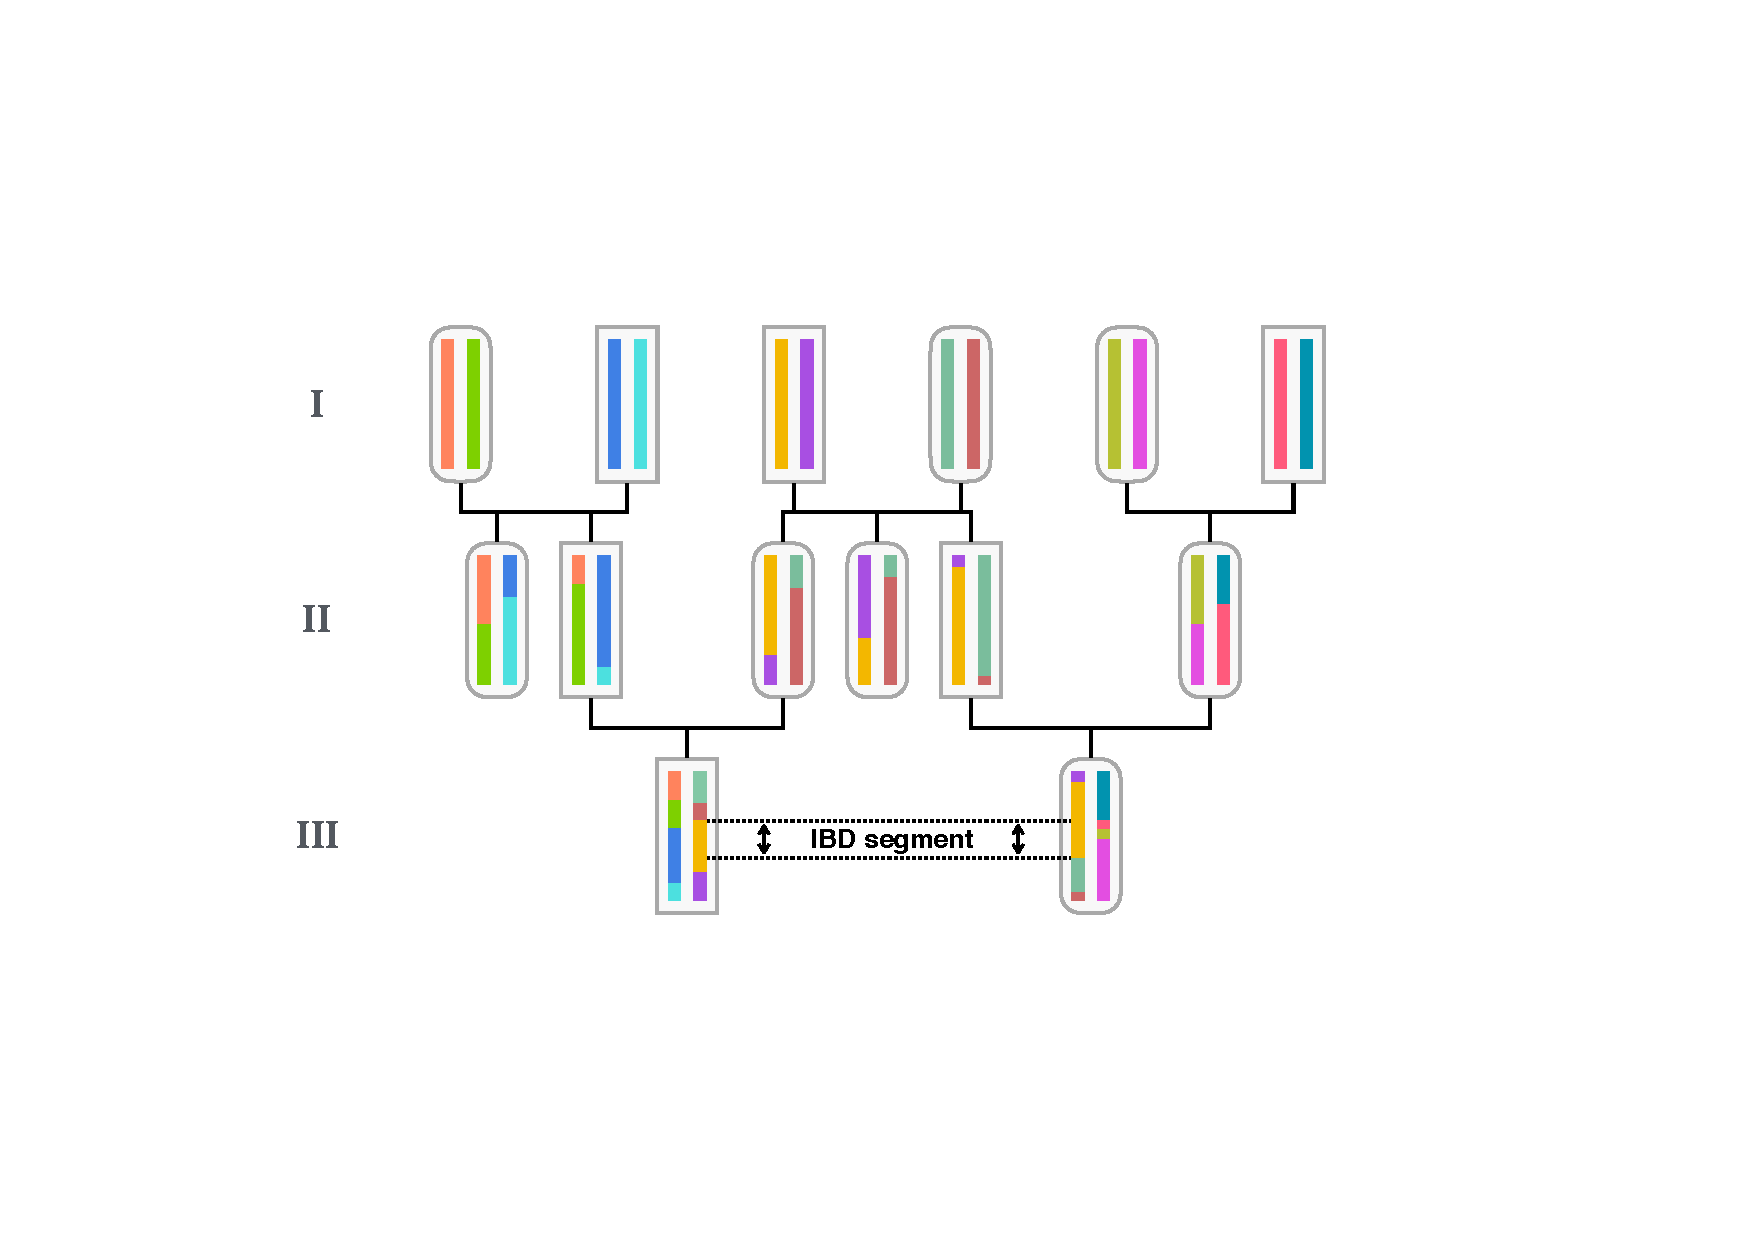
\includegraphics[width=\textwidth]{./img/ch1/info_ibd}
{\small\texthv{\textbf{(b)}}} \\
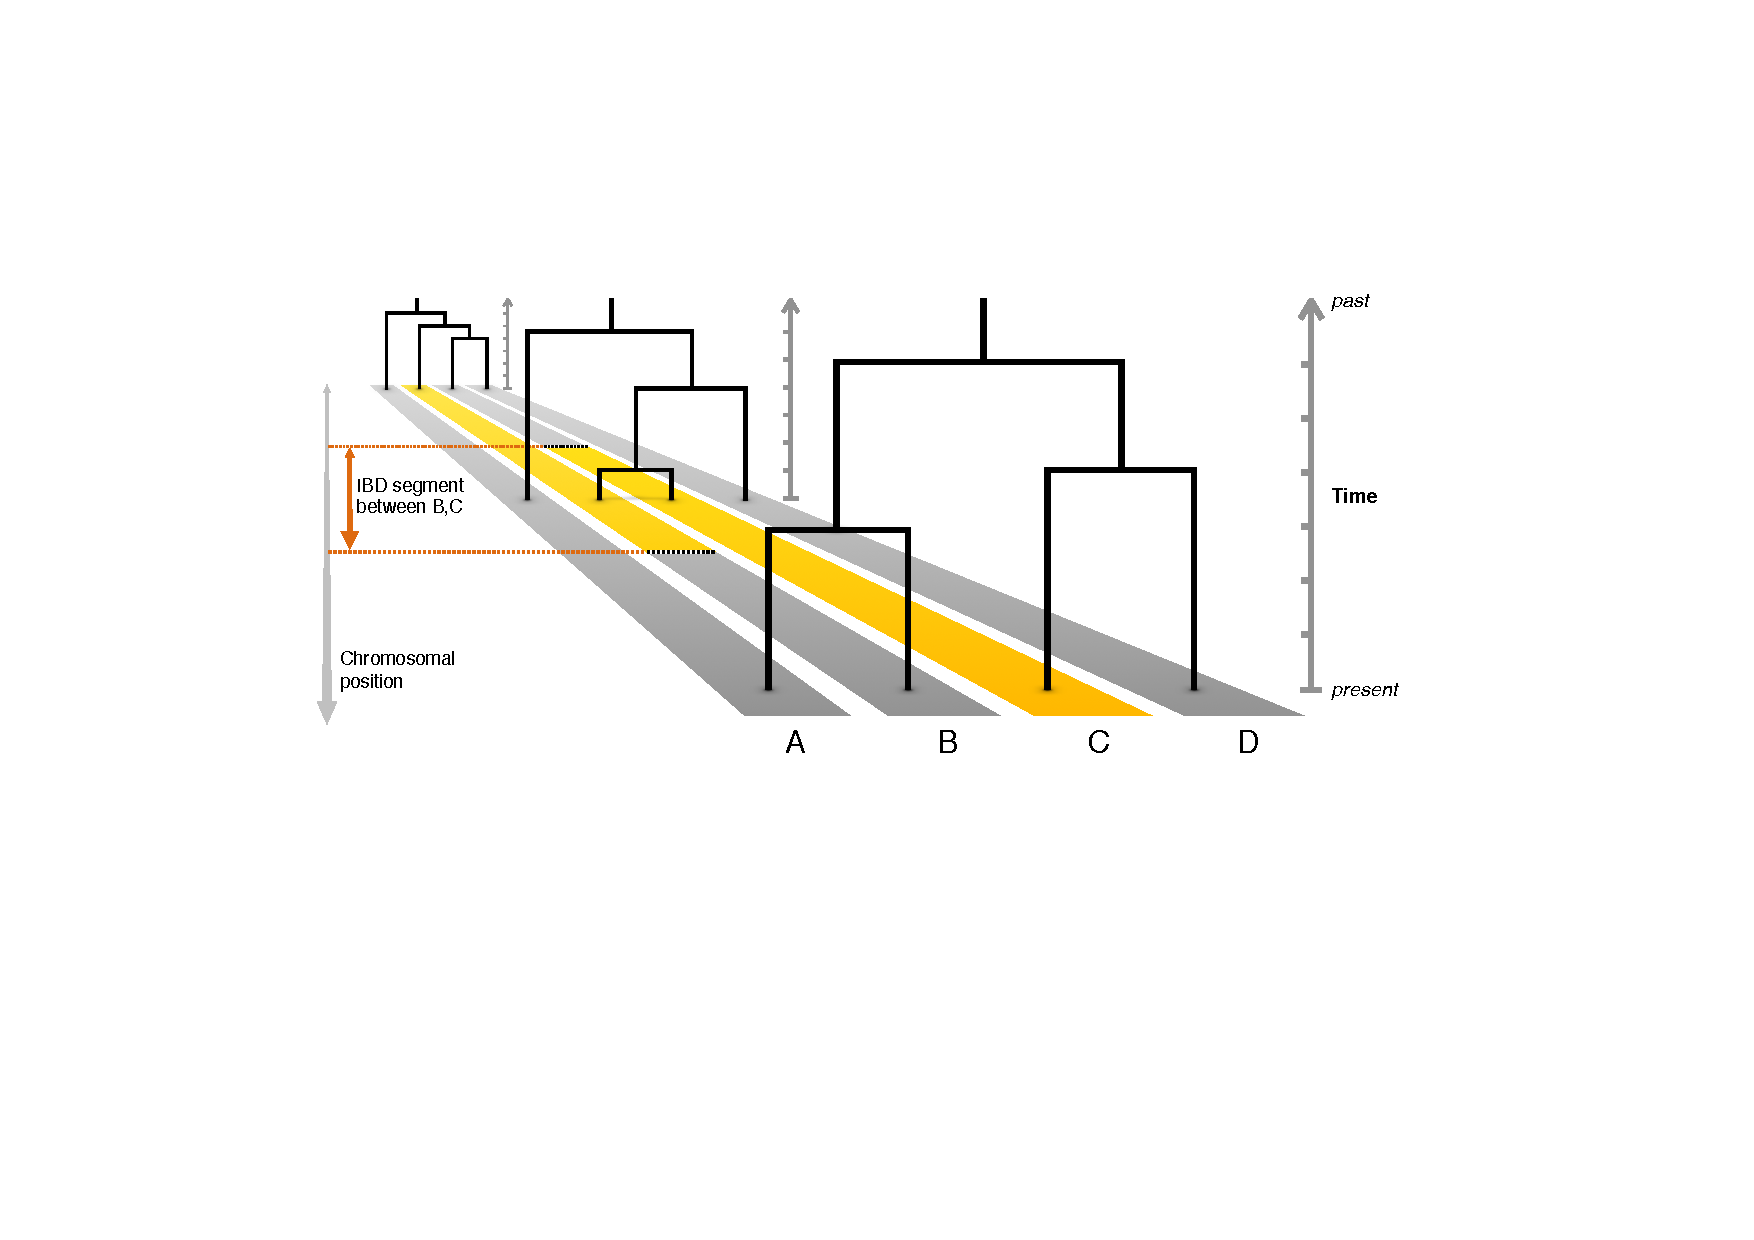
\includegraphics[width=\textwidth]{./img/ch1/info_ibd_segment}
\Caption{Illustration of haplotype sharing by descent}
{Panel~\textbf{(a)} shows a \n{3}-generation pedigree; generation~\rom{1} consists of the founders of the pedigree.
The \n{2} individuals shown in generation~\rom{3} are first-degree cousins.
Male and female individuals are distinguished by square and round shapes, respectively.
Each individual carries a diploid genome, shown as \n{2} large homologous chromosomes.
The colour of each chromosome indicates the ``identity'' of the shared ancestral haplotype, which is shuffled with the other haplotype present in the same individual due to meiotic recombination in each generation, such that the offspring receives a unique arrangement of haplotype segments per chromosome from each parent.
The ``shared'' haplotype refers to the overlapping region of haplotypes that are identical by descent; \ie the IBD segment shared by the \n{2} individuals in generation~\rom{3}, indicated by the \emph{orange} ancestral haplotype.
For simplicity, colours indicate ancestry relative to the founders of the pedigree shown.
Panel~\textbf{(b)} illustrates the different genealogies along the length of the sequence of \n{4} chromosomes (A, B, C, and D), indicated by \n{3} marginal trees.
The IBD segment co-inherited by chromosomes B and C is found at the overlapping region of the shared ancestral haplotype of the \gls{mrca} (\emph{orange}).
Note that the \n{4} chromosomes given in Panel~(b) show a simpler arrangement of haplotypes than shown in Panel~(a).}
{fig:info_ibd}
\end{figure}
